\documentclass[a4paper]{article}
\usepackage[utf8]{inputenc}
\usepackage[T1]{fontenc}
\usepackage[french]{babel}

\usepackage{graphicx}
\usepackage{wrapfig}


\usepackage{changepage}


\usepackage{makecell}
\usepackage{multirow,longtable}
\usepackage{rotating}
\usepackage[table]{xcolor}
\usepackage{booktabs}
\usepackage{array}
\usepackage{geometry}

\begin{document}

\definecolor{headb}{HTML}{1F497D}
\definecolor{lineb}{HTML}{D3DFEE}

\title{
	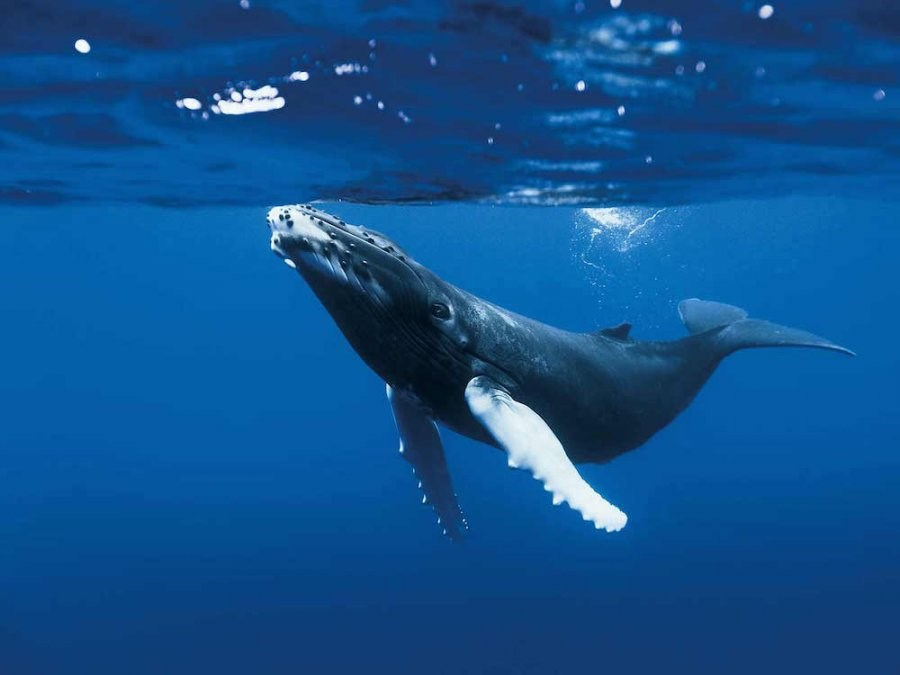
\includegraphics[width=\textwidth]{./tmp/IntroBaleine.png}~\\[1cm]
	\textbf{Projet EBDO} : \textbf{E}xploring \textbf{B}ig \textbf{D}ata \textbf{O}ceans}
\author{ABDALLAH Ghina\\
	\and
	AUREL Cédric\\
	\and
	BAKI Yvan\\
	\and
	DEGURSE Alexandre\\
	\and
	BOUQUET Paul\\
	\and
	MORICONI Florent}

\date{\vspace{-5ex}}
\maketitle
\newpage

\tableofcontents
\newpage

\section{Résumé}
Dans le cadre de notre deuxième année en SPID du cycle ingénieur de l’ENSTA Bretagne, nous
avons réalisé un projet pluridisciplinaire qui a pour but de nous faire découvrir l’organisation et
les méthodes utilisées pour la gestion d’un projet complexe. D’une durée d’un an, cette
expérience permet d’aborder l’ensemble des étapes nécessaires à la réalisation d’un système
complet, de la définition des exigences à la qualification opérationnelle en passant par la
conception de l’architecture physique et sa réalisation tout en travaillant en équipe.
\\

Nous travaillons sur le projet EBDO, Exploring Big Data Ocean, encadré par Dorian
CAZAU et Flore SAMARAN, qui vise à réaliser une plateforme permettant de centraliser, traiter
des enregistrements d’acoustiques sous-marins. L’objectif est proposer aux chercheurs en
biologie marine une plateforme qui simplifie leur travail et leur propose des services
supplémentaires.

\section{Abstract}

In the context of our second year in SPID of the ENSTA Bretagne, we are leading a
pluridisciplinar project which aim to make us discover how to organize and manage complex
projects.
\\

We are working on the EBDO project, Exploring Big Data Ocean, oversighten by Dorian
CAZAU and Flore SAMARAN, aims to realize a platform that centralizes, treats passive acoustic
underwater records.

\section{Remerciements}

Nous tenons tout particulièrement à remercier nos encadrants Mr CAZAU et Mme SAMARAN
ainsi que Mr ALLEMANDOU qui nous a apporter son expertise dont l’aide a été substantielle.

\section{Introduction}

Ce projet SPID a pour but de renforcer notre capacité de travail en équipe, notamment
concernant la prise de décisions collectives et la gestion des conflits, ainsi que le partage des
tâches et la coordination nécessaire pour composer avec les méthodes de chacun. La prise de
responsabilités ainsi que le travail sur un projet commun doivent permettre l’accomplissement
personnel des étudiants.
\\

Les équipes de travail ont été formées selon les choix de sujet classés des étudiants,
formant ainsi des groupes hétérogènes dans le but de renforcer la capacité à travailler avec des
collègues aux méthodes et affinités diverses. L’accent est mis sur la capacité à mener à bien un
projet sur le long terme dans les conditions de travail et d’entente les plus favorables.
\\

Le développement du transport de marchandises par voie maritime – près de 90 % du
trafic international – ainsi que l’intérêt croissant pour les énergies marines renouvelables ont
incité à la mise en place d’études scientifiques pour la compréhension des océans afin d’optimiser
les activités humaines qui s’y trouvent. L’étude de la biodiversité des océans et du réchauffement
climatique permet d’identifier les facteurs destructeurs de l’environnement marin et des espèces
aquatiques. La connaissance précise des océans est également un élément stratégique pour la
France – qui possède la deuxième zone économique exclusive en termes de surface – pour la
surveillance des ressources halieutiques ainsi que pour l’étude de la régulation climatique par les
océans. Ces éléments ont justifié la mise en place d’un projet recherche au sein de l’ENSTA
Bretagne.
\\

Nous nous sommes intéressés au projet EBDO – acronyme de Exploring Big Data from the
Oceans. Ce projet a été proposé par Dorian Cazau – chercheur postdoctoral spécialisé dans
l’analyse de données acoustiques – et Flore Samaran – enseignant-chercheure qui s’intéresse
notamment au suivi des cétacés par des méthodes acoustiques – avec la collaboration de Paul
NGuyen Hong Duc, doctorant sur l’utilisation de machine learning dans le domaine de l’acoustique
sous-marine. Le projet EBDO vise à réaliser une plateforme « proof of concept » de traitement de
données issues des océans. Le volume massif des données ainsi que l’hétérogénéité des sources
sont les problématiques principales à résoudre.
\\

Le projet a été renommé U-PAMtoBOD – acronyme de from Underwater Passive Acoustic
Monitoring to Big Ocean Data – pour souligner que les données issues des hydrophones sont
centrales. Les volumes de données mis en jeu compte tenu du traitement de fichiers audio
amènent des problématiques de stockage et d’optimisation des traitements. Pour répondre à
cette complexité, Joseph Allemandou – consultant big data au sein de la Wikimedia Foundation –
s’est joint au projet pour nous apporter son expertise dans ce domaine récent, notamment
concernant le choix de l’architecture.
\\

La plateforme doit permettre de fournir des services à des utilisateurs experts –
biologistes, chercheurs, etc – dans le but de leur permettre de traiter efficacement leurs données.
Un des objectifs principaux du système est la recherche de corrélations entre différents
paramètres : population de cétacés, conditions environnementales, trafic maritime, etc.
L’utilisation de la plateforme ne doit pas nécessiter de compétences dans le domaine
informatique, une couche d’abstraction entre les problématiques techniques et les besoins
scientifiques doit ainsi être mise en place. Le système proposera une interface utilisateur efficace
pour répondre aux problématiques scientifiques – graphe de points, coefficient de corrélation,
données affichées sur la carte du monde, etc – dans le but de faciliter sa démocratisation au sein
des communautés scientifiques. Ces résultats permettront notamment de déterminer avec une
plus grande précision les effets du changement climatique et des activités humaines sur la
biodiversité des océans.
\\

La modularité du système doit permettre de répondre aux évolutions demandées par les
utilisateurs finaux. La recherche de signaux caractéristiques dans la masse de données doit
permettre aux chercheurs de se concentrer sur les intervalles de temps intéressants, l’affichage
multivariable doit permettre quant à lui une meilleure compréhension scientifique des
phénomènes étudiés. Ces besoins nous ont poussé à concevoir un système complet, tout en
restant cohérent sur notre capacité de travail sur une année.

\section{État de l’art}

Observer les fonds marins et surtout les comprendre a toujours été un enjeu majeur dans le
monde.
\\

L’étude des fonds marins attire aussi bien des scientifiques que des industrielles (notamment
pour le commerce maritime) mais aussi l’armée. Plusieurs techniques ont vu le jour afin
d’explorer les fonds marins, ici nous nous restreindrons à l’étude par analyse des signaux
d’acoustique passive.

\subsection{Méthodes de travail classique des acousticiens}

Les biologistes, afin d’étudier des mammifères sous-marins tels que la baleine Blanche, utilisent
des microphones placés dans des bouées dérivant dans des zones cibles. Par la suite, ils
cherchent des motifs, à la main, qui correspondent à des motifs caractéristiques de l’espèce
recherchée. Cela est réalisé à l’aide de techniques de traitement de signal et ce avec des langages
des programmations tel que Matlab, qui ici est le plus répandu dans la communauté du
traitement du signal. Les enregistrements sonores issus des microphones durent d’ordinaire
plusieurs jours, ils peuvent cependant durer jusqu’à une année entière pour les missions les
plus longues.
\\

« Le travail étant fait à la main il devient très vite difficile de pouvoir écouter tous
ces enregistrements » nous rapportait Flore SAMARAN enseignant-chercheure à l’ENSTA
Bretagne. Il s’agit donc là de l’analyse des signaux acoustique d’origine biologique. On retrouver
des procédées plus ou moins similaires dans d’autres secteurs, par exemple avec l’analyse des
signaux acoustique sous-marin d’origine sismique. Ces méthodes «classiques» requièrent
énormément de travail lorsque les enregistrements sont très longs.

Du témoignages de Flore SAMARAN il vient que :

\begin{itemize}
\item a reconnaissance manuelle sur les données sert à identification évènements.

Limites : travail fastueux, impossibilité de couvrir tous les enregistrements en un temps
relativement cours.

\item Logiciel et langage de programmation est Matlab

Limites : pas interopérable, pas calcul distribué, pas open source, pas très performant en
temps de calcul.

\end{itemize}

\subsection{Projets similaires en cours et leurs lacunes}

Il existe à ce jour quelques projets similaires sur le globe. Chacun de ces projets étant ayant plus
ou moins des approches ou des cibles différentes. Nous pouvons citer :

\begin{itemize}

\item SINAY : plateforme Big Data http://aims.sinay.fr/ qui est un bureau d’étude spécialisé dans
l’environnement marin donc les principales applications d’études sont :

\begin{itemize}

\item Surveillance acoustique passive

\item Qualité de l’eau

\item Détection des mammifères marin...

\end{itemize}

\end{itemize}

Toute fois on peut noter quelques limites à SINAY. En effet, SINAY est :
\begin{itemize}
\item déconnecté des communautés scientifiques, alors que ce sont les chercheurs qui ont l’expertise et qui ont les données.

\item Absences de plateforme en ligne pouvant permettre le traitement par web des données acquis
par une tierce personne.
\end{itemize}

Nous citerons également le projet “DCL System Using Deep Learning Approaches for Land-
Based or Ship-Based RealTime Recognition and Localization of Marine Mammals”:


"Ce projet a pour objectif d’appliquer la localisation et la reconnaissance en temps réel des
mammifères marin en appliquant des algorithmes de Deep Learning et de machine Learning.
Ce projet présente quelque limites notamment l’utilisation de Matlab (pas open source, calcule
non distribué, etc.), et sont concentrés sur du calcul haute performance pour du machine
learning en bioacoustique"

\subsection{Etat de l’art des technologies big data}

Le projet EBDO proposer une solution innovante basée sur des outils Big data open source,
interopérable, scalable etc. Des méthodes performante Deep learning, Machine learning pour
faire parler la donnée. En soit ces méthodes ne sont pas novatrices, car depuis quelques années
les secteurs tels que la Finance, les réseaux sociaux, la santé, le E-commerce, le marketing
digitale ... utilisent des méthodes Big data pour résoudre certains problèmes. Par exemple
Google utiliser les méthodes de big data et machine Learning pour optimiser les résultats qui
s’affichent après une recherche saisie par un utilisateur. De même Facebook s’appuie également
sur ces techniques pour nous suggérer des amis. En 2016 UBER à avouer utiliser des
algorithmes de machine Learning pour fixer des prix aux clients de façon ciblé. On pourrait y
consacrer un chapitre entier pour citer des exemples et la liste ne serait pas exhaustive.
L’innovation dans le projet tient du fait de la mise en œuvre de ces techniques dans l’étude des
signaux acoustiques sous-marin.
\\

Expliquons les grandes lignes de la méthode Big Data.


Effectuer des calculs sur des masses importantes de données demande une puissance de calcul
énorme, supérieurs à celle de la plupart des ordinateurs que nous avons au quotidien (scalabilié
verticale). On va utiliser plusieurs ordinateurs de puissance relativement faibles mis en réseau
au moyen des clusters via un système de partage de fichier pour effectuer des calculs
(scalabilité horizontale) : On parle de calcul distribué.
\\

Pour réussir la mise sur pieds d’un tel système il existe des technologies telles que HADOOP,
SPARK, STORM, ELASTICSEARCH, SPARK. Tous ces outils jouent un rôle précis allant du
découpage des fichiers par HADOOP, l’application des calculs souhaités sur ces fichiers
découpés par SPARK en passant par ELASTICSEARCH qui se charge d’effectuer les requêtes sur
le système de fichier distribué. La liste des outils liées à l’environnement Big Data cité ici et
leurs rôles est non exhaustive.
\\

En outre les traitements de ces données par les algorithmes de machines learning et deep
learning s’appuierons sur des bibliothèques déjà existante telles que SPARK MLlib, H20,
Tensorflow etc ...
\\

Tout ceci offre un point d’appui solide pour le départ et la réalisation du projet et permet
d’intégrer toute la chaine de traitement.

\section{Ingénierie système}

\subsection{Exigences du système}

!!! TABLEAU ICI !!!



\subsection{Analyse Fonctionnelle}

A partir des exigences, nous avons établit les fonctions principales du système :

\begin{itemize}

\item Servir des données calculées à partir de gros volume de données brutes
d’acoustique (FP1)

\item Servir des données auxiliaires en les corrélant à des données traitées. (FP2)

\item Stocker les données (FC1)

\item Ingérer des données hétérogènes(FC2)

\item Ingérer des gros volumes de données(FC3)

\item Plateforme doit être ergonomique (FC4)

\item Plateforme doit être Esthétique (FC5)

\item Respecter le prix (FC6)

\item Plateforme doit être sécurisé, libre d’accès et compatible(FC7)

\item Rapidité de calcul et d’ingestion de données(FC8)

\end{itemize}

\newpage
\subsection{Diagramme Pieuvre}

\begin{figure}[h]
	\centering
	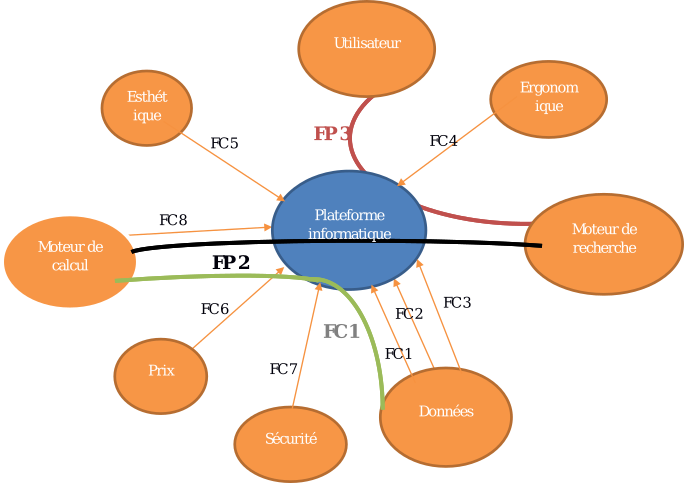
\includegraphics[width=0.9\textwidth]{./tmp/DiagPieuvre.png}
	\caption{Diagramme pieuvre du système}
\end{figure}
\newpage
\newgeometry{left=1cm, top=2cm}
Nous avons également décrit les fonctions du système sous la forme du tableau des fonctions :
\definecolor{headb}{HTML}{1F497D}
\definecolor{lineb}{HTML}{D3DFEE}
%\setlength\LTleft{-3cm}
	\begin{longtable}{|p{1cm}|p{3cm}|p{6cm}|p{5.5cm}|p{30px}|}
        \hline
        \rowcolor{headb}
	{\color{white}ID} & {\color{white}Type} & {\color{white}Expression} & {\color{white}Raison d'être} & {\color{white}Priorité} \\
        \hline
        FP1 & Fonction principale & Servir des données calculées à partir de gros volume de données brutes d’acoustique & & \cellcolor{white} \\\cline{1-3}
        \rowcolor{lineb}
        FP11 & Fonction auxiliaire & Ingérer les données acoustiques brutes &\cellcolor{white} & \cellcolor{white} \\\cline{1-3}
        FP111 & Fonction auxiliaire & Extraire les métadonnées utiles lors de l'ingestion & \cellcolor{white} & \cellcolor{white} \\\cline{1-3}
        \rowcolor{lineb}
        FP112 & Fonction auxiliaire & Stocker les données brutes & \cellcolor{white} & \cellcolor{white} \\\cline{1-3}
        FP12 & Fonction auxiliaire & Effectuer les traitements sur les données brutes & \cellcolor{white} & \cellcolor{white} \\\cline{1-3}
        \rowcolor{lineb}
	FP13 & Fonction auxiliaire & Stocker les données calculées & \cellcolor{white} \cellcolor{white}\makecell[c]{\cellcolor{white} Fournir à l'u\-ti\-li\-sa\-teur\\ le service de\-man\-dé} & \cellcolor{white} \multirowcell{-2}{3} \\\cline{1-3}
        FP14 & Fonction auxiliaire & Servir les données traitées à travers un serveur web & \cellcolor{white} & \cellcolor{white} \\\cline{1-3}
        \rowcolor{lineb}
        FP141 & Fonction auxiliaire & Saisir la requête de l'utilisateur et servir les données correspondantes & \cellcolor{white} & \cellcolor{white} \\\cline{1-3}
	FP142 & Fonction auxiliaire & Intégrer les données obtenues à une visualisation adéquate & & \\\cline{1-3}\cline{5-5}
        \rowcolor{lineb}
	FP2 & Fonction principale & Servir les données auxiliaires en les corelant à des données traitées & \cellcolor{white} & 2 \\\hline
        FP21 & Fonction auxiliaire & Ingérer des données auxiliaires & \cellcolor{lineb} & 2 \\\cline{1-3}
        \rowcolor{lineb}
	FP22 & Fonction auxiliaire & Stocker les données auxiliaires & \makecell[l]{Posséder plus d'information pour\\une meilleure compréhension\\de certains phénomènes\cellcolor{lineb}} & 2 \\\hline
        FP23 & Fonction auxiliaire & Saisir la requête de l'utilisateur & Servir un ensemble personnalisé d'informations & 2 \\\hline
        \rowcolor{lineb}
        FP24 & Fonction auxiliaire & Corréler les données auxiliaire aux données calculés sur la base de la requête de l'utilisateur & Préparé les données pour une future requête utilisateur & 2 \\\hline
        FP25 & Fonction auxiliaire & Servir les données correspondantes & Respecter la demande de l'utilisateur & 2 \\\hline
        \rowcolor{lineb}
        FP26 & Fonction auxiliaire & Intégrer les données obtenues à une visualisation adéquate & Permettre à l'utilisateur une meilleure compréhension         & 1 \\\hline
        FC1 & Fonction contrainte & Stocker les données & (vide) & 2 \\\hline
        \rowcolor{lineb}
        FC2 & Fonction contrainte & Ingérer des données hétérogènes & & 1 \\\cline{1-3}
	FC3 & Fonction contrainte & Ingérer des gros volumes de données & \cellcolor{lineb}\makecell[c]{Permettre une certaine\\flexibilité à l'utilisateur} & 2 \\\hline
        \rowcolor{lineb}
        FC4 & Fonction contrainte & Être ergonomique &\cellcolor{white} & 1 \\\cline{1-3}
	FC5 & Fonction contrainte & Être esthétique & \makecell[c]{Fournir un espace de travail\\ conviviale et facile d'utilisation} & 1 \\\hline
        \rowcolor{lineb}
        FC6 & Fonction contrainte & Respecter le prix & Le client désire réduire le coût de la réalisation & 3 \\\hline
        FC7 & Fonction contrainte & Être securisé, libre d'accès et compatible & L'utilisateur désire une disponibilité et une sécurité optimale & 3 \\\hline
        \rowcolor{lineb}
        FC8 & Fonction contrainte & Limiter le temps de calcul & Réduire le temps d'attente de l'utilisateur & 2 \\\hline

	\caption{Fonctions du système}
\end{longtable}
\restoregeometry

\newpage
\subsection{Diagramme FAST}

\begin{figure}[h]
	\centering
	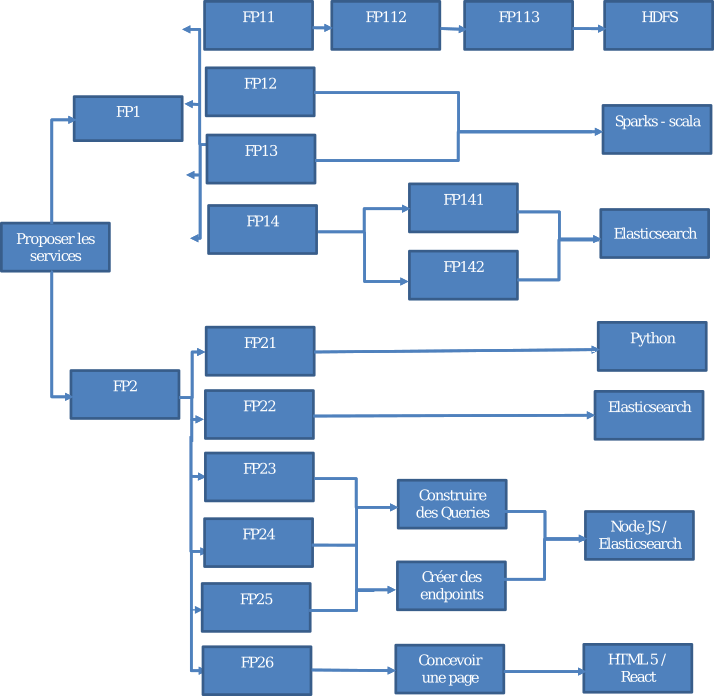
\includegraphics[width=\textwidth]{./tmp/DiagFast.png}
	\caption{Diagramme FAST du système}
\end{figure}

\newpage
\subsection{Chaine fonctionnelle}

\textbf{FP1} : Servir des données calculées à partir de gros volume de données brutes d’acoustique.

\begin{figure}[h]
\centering
	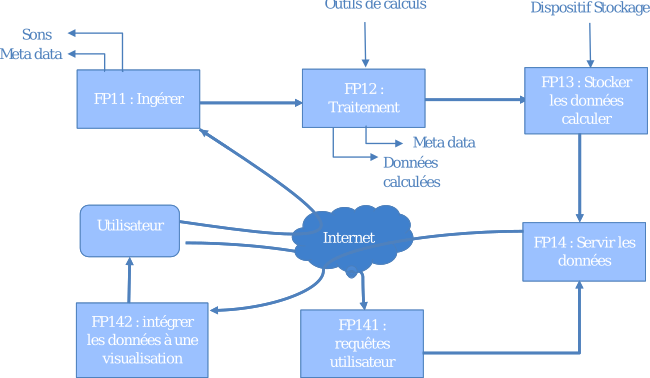
\includegraphics[width=0.8\textwidth]{./tmp/ChaineFonct.png}
	\caption{Chaine fonctionnelle FP1}
\end{figure}

\textbf{FP2} : Servir des données auxiliaires en les corrélant à des données traitées.

\begin{figure}[h]
\centering
	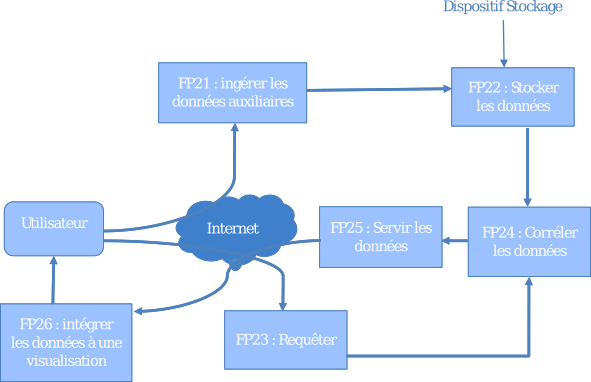
\includegraphics[width=0.8\textwidth]{./tmp/ChaineFonct2.png}
	\caption{Chaine fonctionnelle FP2}
\end{figure}

\newpage
\subsection{Architecture Physique}

Afin de répondre au mieux aux exigences nous avons défini l’architecture physique
préliminaire suivante, en commençant par les sous-systèmes que nous avons identifiés :

\begin{itemize}

\item Sous-système d’ingestion de données

\item Sous-système de stockage des données massive

\item Sous-système de traitement des données massives

\item Sous-système de stockage des données traités et auxiliaires

\item Sous-système de serveur web

\item Sous-système de visualisation web

\end{itemize}

\begin{figure}[h]
	\centering
	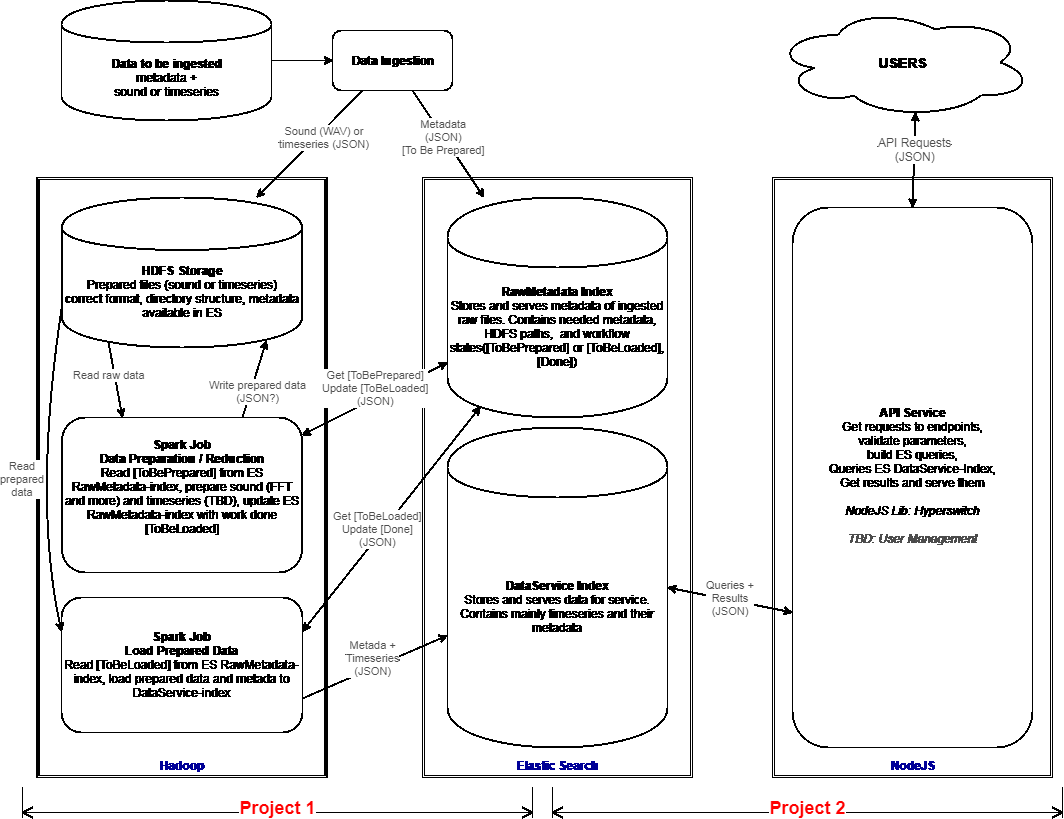
\includegraphics[width=\textwidth]{./tmp/ArchiPhy.png}
	\caption{Détails de l'architecture physique}
\end{figure}

\section{Conduite de projet}

\subsection{Environnement de travail collaboratif}

Ce projet est un travail collaboratif, l’équipe est un groupe de 6 étudiants. Chacun de ces étudiants
à un rôle spécifique. Le tableau ci-dessous présente le rôle de chaque membre au sein du projet,
c’est-à-dire sur quel sous-projet il travaille.

	\begin{table}[!h]

\begin{center}
	\begin{tabular}{|l|c|}

\hline
        \rowcolor{headb} \multicolumn{1}{|c|}{{\color{white}\'Etudiant}}  & {\color{white}Sous-projet}\\
\hline
        \rowcolor{lineb}
        ABDALLAH Ghina          & Middleware\\
        BAKI Yvan               & Backend\\
        \rowcolor{lineb}
        BOUQUET Paul            & Backend\\
        MORICONI Florent        & Middleware\\
        \rowcolor{lineb}
        SONGO SONKENG Cedrice Aurel & Middleware\\
        DEGURSE Alexandre       & Middleware\\
        \hline
\end{tabular}

	\caption{Répartition de l'équipe}

\end{center}
\end{table}

Même si nous ne travaillons pas tous sur la même partie du projet, nous avons eu besoin de mettre
en place des outils de travail collaboratif afin d’être efficace.

\subsection{Répartition et suivi du travail}

Le premier défi en terme de collaboration est la répartition du travail et le suivi du travail de
chaque membre du groupe. Afin de pouvoir savoir où en est chacun et d’éviter un blocage dans
l’avancement du projet, nous avons choisi Trello. Dans celui-ci, tout y est présenté graphiquement
sous forme de «cartes » qui permettent de suivre l’avancement objectifs fixés à chaque personne
mais aussi de revoir en détail quels étaient ces objectifs.
\\

On divise ainsi le travail en cartes, ces cartes sont censées pouvoir être réalisés en une à deux
semaines. Dans chaque carte, on renseigne une description globale ainsi que plusieurs sous-
tâches qui représentent chacune un volume de travail plus faible. Une carte est donc considérée
réalisée lorsque toutes les sous-tâches ont été réalisées. On peut cocher les sous-tâches une fois
accomplies afin de faire progresser l’avancement de la carte (voir Figure \ref{CarteTrello}).
\\

On peut aussi gérer les cartes à un niveau supérieur sur le tableau où elles sont affichées (voir Figure \ref{TabTrello}).
On peut les placer dans des colonnes qui représentent l’état de la carte. Nous avons
défini plusieurs états : Proposition, To do, Technical design (pour la cherche de solutions afin de
commencer le travail), Ongoing, CodeReview (évaluation du travail effectué par les autres
membles du groupe) et Done.

\begin{figure}[!htb]
   \begin{minipage}{0.48\textwidth}
     \centering
     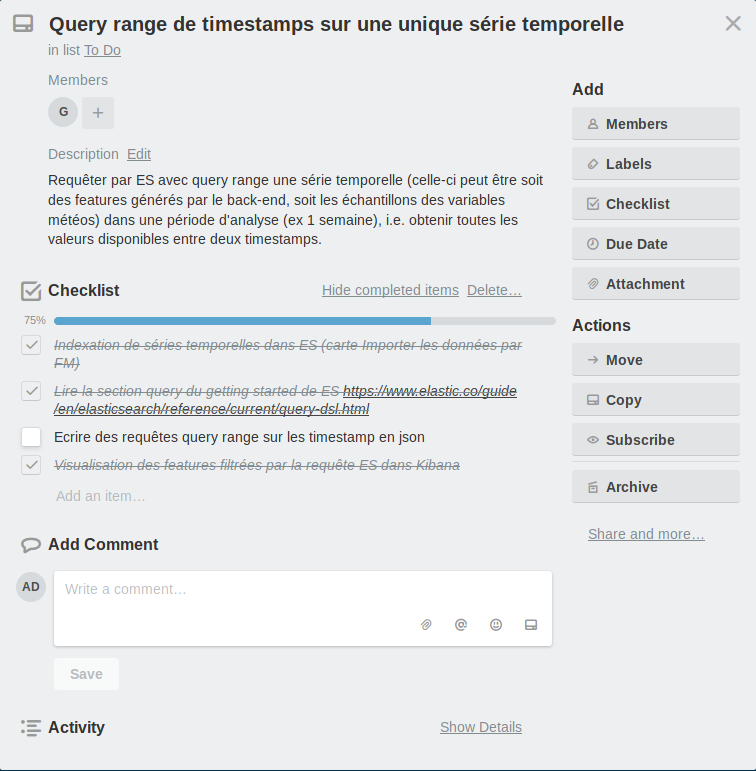
\includegraphics[width=.7\linewidth]{./tmp/CarteTrello.png}
	   \caption{Détails d'une carte de Trello\label{CarteTrello}} 
   \end{minipage}\hfill
   \begin {minipage}{0.48\textwidth}
     \centering
     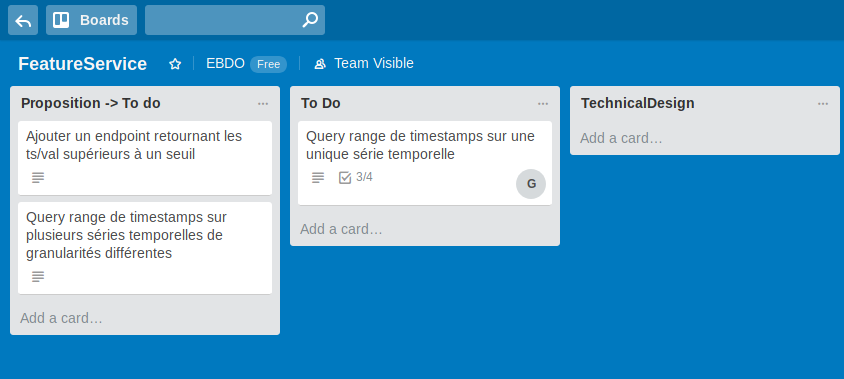
\includegraphics[width=.7\linewidth]{./tmp/Trello.png}
	\caption{Aspect général de Trello\label{TabTrello}}
   \end{minipage}
\end{figure}

\newpage
\subsection{Communication dans le groupe}
\begin{figure}[h]
\begin{minipage}{.48\textwidth}
%\begin{wrapfigure}{l}{150px}
	\centering
	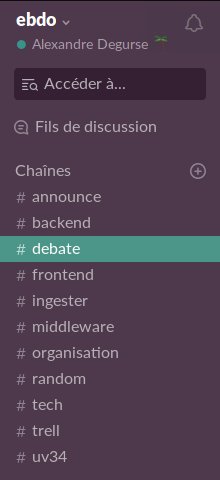
\includegraphics[width=200px]{./tmp/ChanSlack.png}
	\caption{Exemple de channel}
%\end{wrapfigure}
\end{minipage}
\begin{minipage}{.48\textwidth}

La communication et les échanges entre les différents
membres de l’équipe est étant primordiale dans un
projet collaboratif. Nous avons choisi Slack comme une
plate-forme de communication.
\\

Il nous permet de simplifier et de mieux organiser nos
échanges. Nous avons la possibilité de créer des
chaînes de discussions afin d’organiser les messages
mais aussi de suivre facilement le fil des discussions
concernant chaque partie du projet.
\\

Slack permet aussi de « poker » une personne, en
écrivant @’’nom’’, cela permet de l’interpeller en lui
envoyant un mail de notification. Cela est utile afin
d’être réactif quand nécessaire.
\end{minipage}
\end{figure}


\newpage
Ci-dessous, un exemple de fil de discussion Slack.
\begin{figure}[!h]
\centering
	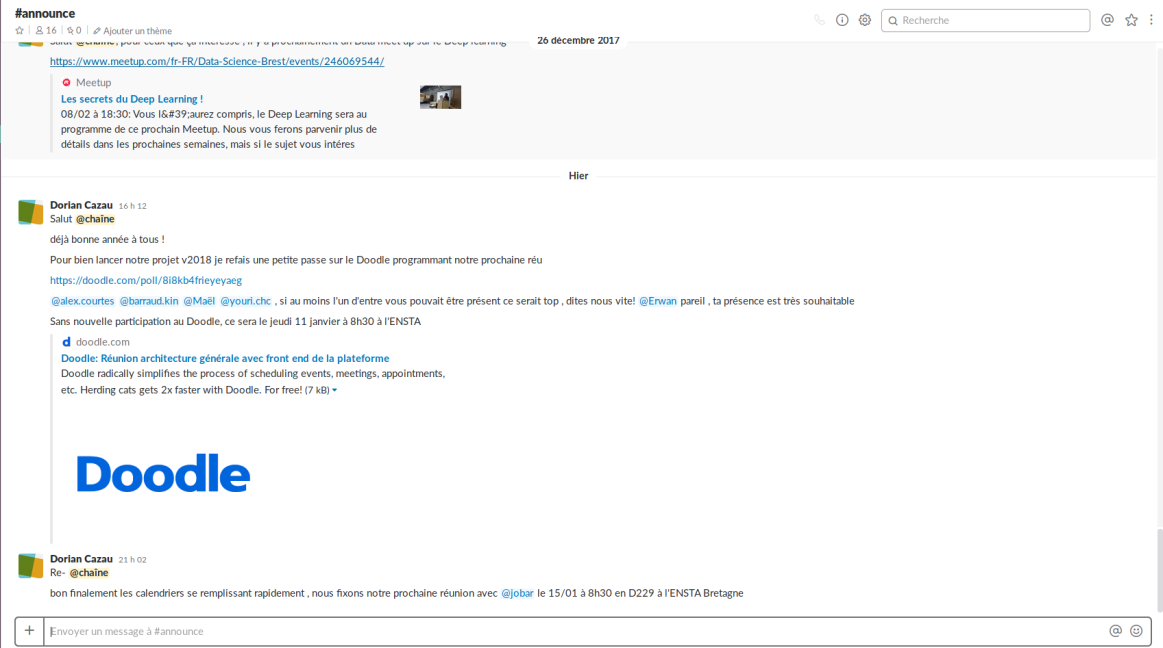
\includegraphics[keepaspectratio, height=150px]{./tmp/ChatSlack.png}
\end{figure}

\subsection{Partage du travail}

Enfin, sûrement l’une des plus grosses difficultés, le partage du travail.


Plusieurs personnes interviennent dans développement et d’écriture du code d’un sous-projet.
Cela peut poser de gros problèmes si l’on n’utilise pas des outils adéquats. Par exemple, si deux
personnes modifient une même portion du code existant, cela va poser des problèmes lorsque
leurs travaux vont être fusionnés. Il est possible de gérer ‘à la main’ ces problèmes, mais cela
nécessite beaucoup de travail lors qu’il faut regrouper le travail de chacun. Les logiciels de gestion
de version sont destinés à surmonter ces difficultés. Ils fournissent un système de fusion de code
très puissant mais aussi un système d’historique de version. Cela consiste à renseigner l’utilité de
chaque nouvelle version. Cela peut être coûteux au début mais après plusieurs mois, on peut
facilement retrouver pourquoi chaque bloc de code a été ajouté.
\\

Nous avons choisi Git/Github comme logiciel de gestion de version. Ainsi, chacun parmi nous
travaille sur une copie du code sur son propre ordinateur, apporte des modifications, puis quand
il juge que sa version est satisfaisante, il la transmet à Github, qui centralise les modifications en
ligne. A partir de là, les autres membres du groupe peuvent récupérer le code et le fusionner avec
le leur.

\subsection{Relation client}

Nous planifions une réunion de projet par semaine. Avant la réunion, nous préparons et envoyons
l’ordre du jour de la réunion qui contient les points à aborder. Durant la réunion, nous ne
discutions pas que les points déjà qui sont déjà écrites dans l’ordre, mais aussi d’aborder des
sujets importants pour notre encadrant ou Mme Samaran. Nous profitons de ces occasions pour
coordonner et recentrer le travail sur le retour que nous font nos encadrants. Il s’agit de présenter
le travail que nous avons effectué et de voir à quel point celui-ci abonde dans le sens des
exigences.

\subsection{Relation avec un consultant extérieur}

Un expert technique, dans le domaine des bases de données distribuées, Joseph
ALLEMANDOU nous assiste dans le projet pour nous donner des conseils techniques et nous aider
à résoudre les problèmes auxquels nous sommes confrontés durant le développement.

\subsection{Atelier technique}

À l’occasion des ateliers techniques, notre encadrant à organiser un atelier Traitement de
données massives. Joseph Allemandou est intervenu à cette occasion pour nous présenter les
enjeux et les technologies dans ce domaine. Cet atelier nous a apporté des connaissances
techniques primordiales ainsi qu’une meilleure vision d’une partie du système. Nous avons, à
cette occasion, acquis les bases du traitement de données massives distribué à l’aide du
Framework Apache SPARK, le Framework utilisé pour la partie backend.

\subsection{Méthodes Agiles}

Afin de mener à bien le projet, nous avons mis en place des principes issus du management
AGILE.
\\

Cela est marquant en ce qui concerne la proximité avec les client grâce aux réunions. Nous
essayons de faire en sorte de faire avancer le projet de façon à ce qui le client voit rapidement
les premières fonctionnalités du système. Ainsi, nous avons son retour immédiat sur ce qui a été
implémenté puisque qu’il peut tester. Sur la base du retour du client sur la fonctionnalité, nous
corrigeons ce qui ne lui convient pas et améliorons les points qui peuvent l’être.
\\

De plus, les nombreux outils collaboratifs que nous avons mis en place nous permettent de
synchroniser notre travail et de faire avancer le projet petit à petit par version successive. Cela
permet de mieux organiser le travail, de mieux mesurer l’avancement du développement et
donc d’être plus efficace.

\section{Conclusion}

L’efficacité des outils de collaborations mis en place ainsi que la programmation de
réunions bihebdomadaires nous a permis une productivité accrue. Les premiers codes utiles à la
plateforme finale sont en cours d’intégration dans les répertoires officiels. Le fonctionnement du
backend et du middleware sur des données de faible volume est une réalité. L’ajout progressif de
fonctionnalités pour satisfaire l’ensemble des exigences permet dès à présent des usages simples
sur une chaine de traitement complète.
\\

Dans un futur proche, les premiers essais de mise à l’échelle auront lieu sur Datarmor –
supercalculateur appartenant à l’IFREMER – pour permettre de valider les solutions
technologiques retenues, notamment concernant le backend.
\\

La mise en place d’une collaboration avec une dizaine d’étudiants de l’EPSI – école
d'ingénierie en informatique située à Kergaradec – doit permettre le développement simultané
du frontend de la plateforme. Ce partenariat requiert la mise en place d’une coordination inter-
écoles et implique particulièrement la définition précise des exigences nécessaires à
l’aboutissement d’un produit de qualité.
\\

Le machine learning est un axe majeur de développement du projet afin de faciliter le
traitement de grand volume de données. L’identification de motifs dans les données permettrait
aux scientifiques de se focaliser sur les intervalles spatio-temporels intéressants. Les nombreux
développements prévus laissent à penser que ce projet pourrait sortir du cadre de la recherche
pour se muer – avec le soutien de l’incubateur de l’ENSTA - vers un modèle de fournisseur de
service.

\listoffigures

\listoftables

\end{document}
